\chapter{Realisierung}
\label{sec:realisierung}

In diesem Kapitel werden die im vorherigen Kapitel beschriebenen Konzepte anhand eines Prototypen implementiert. Die konkrete Logik wird bei jedem implementierten Konzept anhand von Code erläutert.

\section{Eingesetzte Technologien}

Für die Entwicklung des Prototyps kamen folgende Technologien zum Einsatz:

\begin{itemize}
	\item Als Game-Engine wurde Unity benutzt. Die Entscheidung hierfür begründet sich durch die gute Dokumentation und den Long-Time-Support der verschiedenen Unity-Versionen \cite{Technologies.03.02.2022}. Außerdem gibt es eine große Anzahl von Benutzern. Unity existiert bereits seit 2005 und hat sich seitdem in Entwickler-Kreisen einen nachhaltigen Ruf erarbeitet \cite{W.LinLin.2017}.
	\item C\# kommt als Programmiersprache zum Einsatz. Unity bietet eine sehr gute Unterstützung hierfür.
	\item Zusätzlich zu Unity wurde Mirror als weiteres Framework benutzt. Mirror ist eine kostenlose Open Source Networking Bibliothek, welche die Entwicklung von Netzwerk-Code deutlich erleichtert \cite{.03.02.2022}.
\end{itemize}

\section{Spielidee des Prototyps}
\label{Spielidee}

Das Grundprinzip des Prototyps basiert auf dem Kinderspiel 'Fangen und Verstecken'. Hinzu kommen weitere Spiel-Elemente, die in dieser Sektion erläutert werden. Innerhalb der Spielwelt existieren 2 verschiedene Teams, die ausschließlich aus Spielern bestehen.

Spieler mit der Rolle 'Hider' und 'Ghost' gehören zu einem Team.  Spieler mit der Rolle 'Seeker' bilden das zweite Team. Anfangs wird per Zufall entschieden, welche Spieler zum Team 'Hider/Ghost' und welche zum Team 'Seeker' gehören. Alle Teammitglieder des Teams 'Hider/Ghost' beginnen das Spiel initial als 'Hider'. Der Leiter einer Lobby kann festlegen, ob ein oder zwei Seeker ausgewürfelt werden sollen. Zum Leiter einer Lobby wird derjenige Spieler, der als Erstes einer Lobby beitritt. Sollte der Leiter einer Lobby diese verlassen, wird der Spieler zum Leiter, der am längsten Mitglied derselben Lobby war. Die Aufgaben der Spieler sind je nach Rolle unterschiedlich:

\textbf{Hider:} \\
Spieler mit der Rolle 'Hider' haben die Aufgabe, bestimmte Objekte in der Spielwelt zu finden und diese zu einem Zielort zu bringen. Sind alle Objekte zu ihrem Zielort gebracht, so hat das Team 'Hider/Ghost' das Spiel gewonnen. Hider müssen zudem vor den Spielern mit der Rolle 'Seeker' flüchten, bzw. sich vor diesen verstecken. 

\textbf{Seeker:} \\
Spieler mit der Rolle 'Seeker' haben lediglich eine Aufgabe. Sie müssen alle Spieler mit der Rolle 'Hider' fangen. Dies können sie tun, indem sie in die unmittelbare Reichweite eines Hiders laufen und die Taste 'E', oder den in der Benutzeroberfäche festgelegten Knopf 'Catch', drücken. Sind alle Hider gefangen, so gewinnen die Seeker das Spiel.

\textbf{Ghost:} \\
Spieler, die initial mit der Rolle 'Hider' gespawnt sind und von einem Seeker gefangen wurden, wechseln ihre Rolle zu 'Ghost'. Ghosts dürfen nicht mehr mit Objekten der Spielwelt interagieren, sie können sich lediglich noch über das Spielfeld bewegen. Außerdem bekommt ein Ghost eine Fähigkeit, die er einsetzen kann, um seinem Team zu helfen. Diese Fähigkeit ermächtigt den Spieler, einen Seeker für 3 Sekunden bewegungsunfähig zu machen, sollte der Spieler in der unmittelbaren Nähe eines Seekers sein und die Taste 'E', bzw. den dafür vorgesehen Knopf in der Benutzeroberfläche drücken. Diese Fähigkeit kann lediglich alle 30 Sekunden eingesetzt werden.

Das Spielkonzept wird in folgendem Spielflussdiagramm zusammengefasst:

\begin{figure}[H]
	\centering
	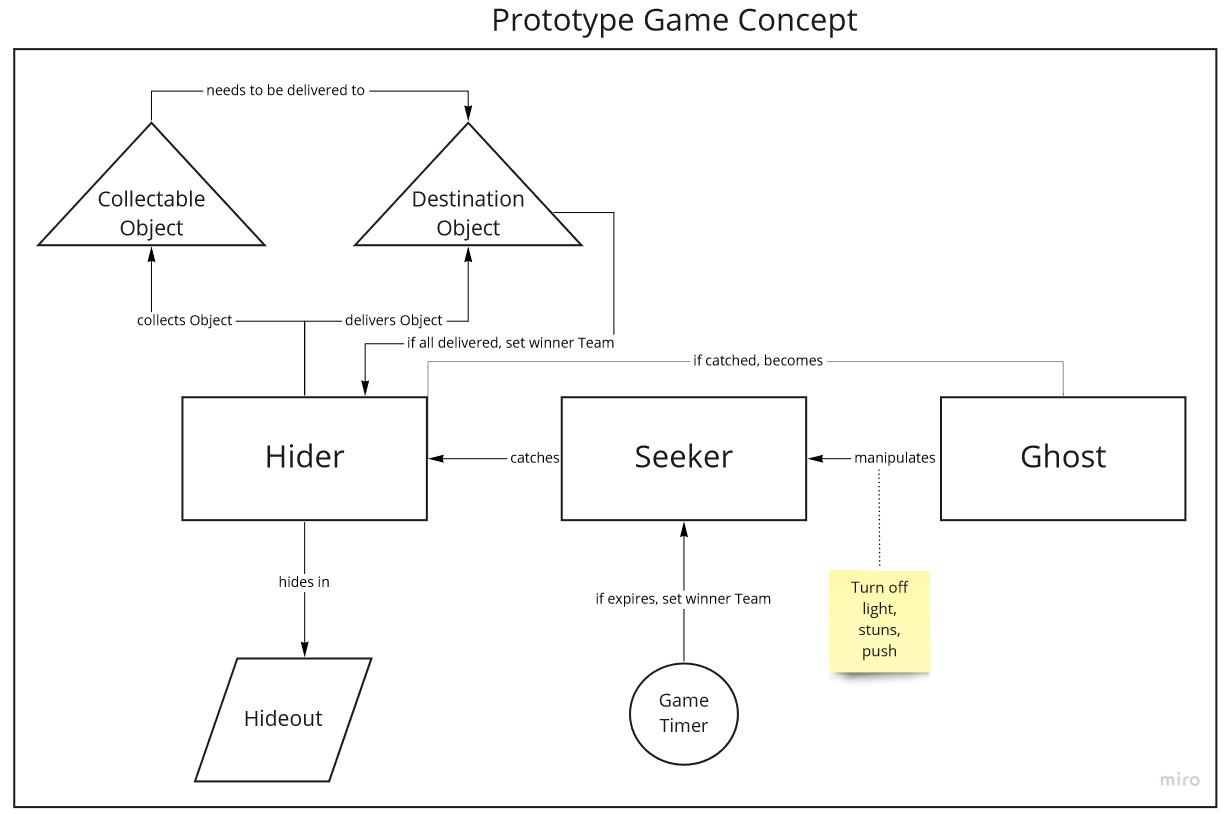
\includegraphics[width=115mm]{images/game_concept.jpg}
	\caption[Spielkonzept Diagramm]{Veranschaulichung des Spielkonzepts}
	\label{pic:game_concept}
\end{figure}

\textbf{Spiel-Ablauf:}

Zunächst muss ein Spieler eine Lobby erstellen. Dies tut er, indem er auf den Knopf 'Create Lobby' im Hauptmenü drückt. Nun erhält dieser Spieler einen 'Code', der eindeutig diese Lobby identifiziert. Diesen 'Code' kann der Spieler jetzt an seine Mitspieler weitergeben. Diese können den Code im Hauptmenü in ein Eingabefeld eingeben und auf 'Join Lobby' drücken. Der Spieler, der die Lobby erstellt hat, ist inzwischen auch Lobbyleiter und kann einstellen, ob die Lobby als 'public' markiert werden soll. In diesem Fall können andere Spieler durch den Button 'Join Random Lobby' ebenfalls der Lobby beitreten, ohne den Code zu kennen. Das folgende Aktivitätsdiagramm zeigt die möglichen Abfolgen des Beitritts einer Lobby:

\begin{figure}[H]
	\centering
	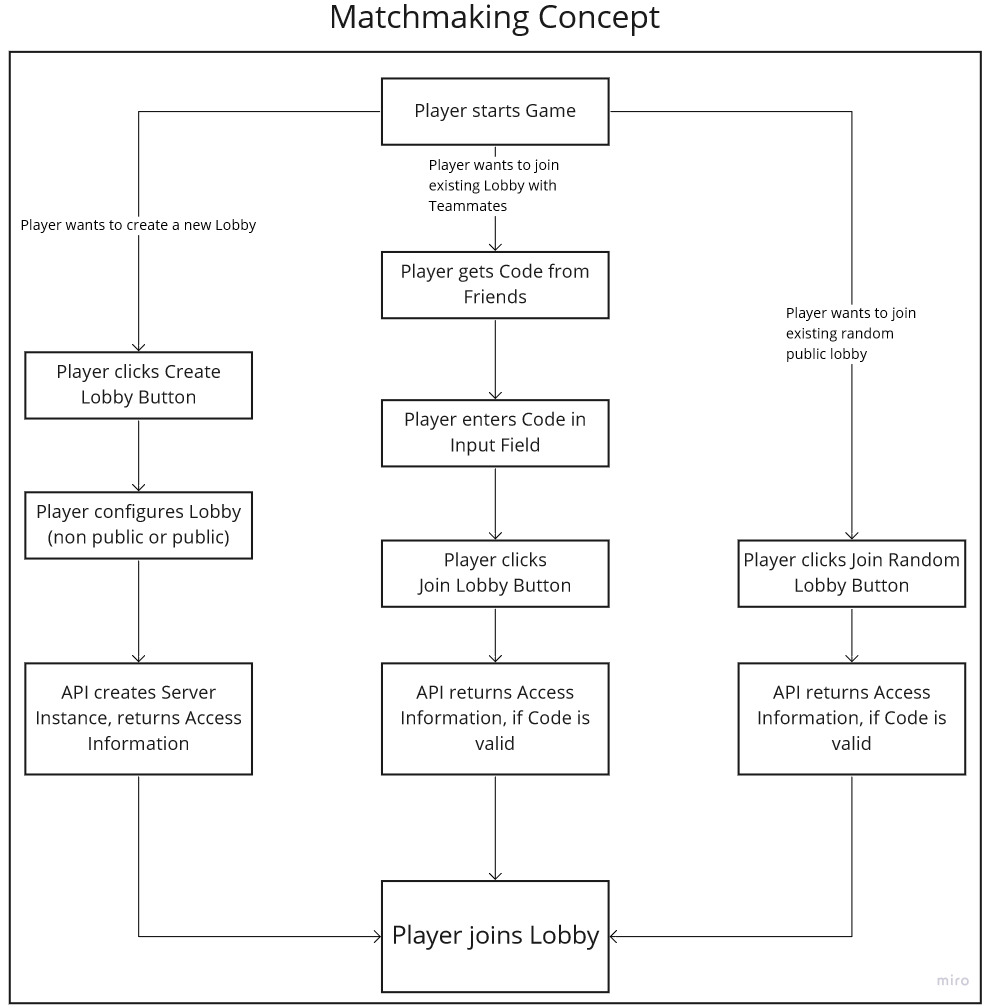
\includegraphics[width=110mm]{images/matchmaking_concept.jpg}
	\caption[Matchmaking-Konzept Diagramm]{Veranschaulichung des Prototyp-Matchmaking}
	\label{pic:matchmaking_concept}
\end{figure}

Ist nun eine Lobby erstellt und es sind mindestens 2 und maximal 10 Spieler der Lobby beigetreten, die ihren Bereitschaftsstatus durch das Drücken des Knopfes 'Ready' kommuniziert haben, so hat der Lobbyleiter die Möglichkeit, durch Drücken des Buttons 'Start Game' das Spiel zu starten.

Aus insgesamt 10 möglichen Spawn-Punkten würfelt der Prepare-Game-Manager Spawn-Punkte für die beigetretenen Spieler aus. Sobald alle Spieler die Spiel-Szene geladen haben und auf ihren Startpunkten stehen, beginnt das Spiel. Ab diesem Zeitpunkt läuft eine Stoppuhr ab. Erreicht diese den Wert '0' bevor alle Objekte an ihren Zielort gebracht wurden, so hat das Team 'Seeker' gewonnen.

\section{Architektur des Prototyps}
\label{Architektur}

\textbf{Matchmaking:} \\
Die Matchmaking Architektur basiert auf einem Client Server Modell, sowie dem Einsatz einer REST API, die als Matchmaking- und Server-Runner Schnittstelle dient. Der oben beschriebene Ablauf zum Beitreten einer Lobby ist im folgenden Diagramm noch einmal aus technischer Sicht visualisiert:

\begin{figure}[H]
	\centering
	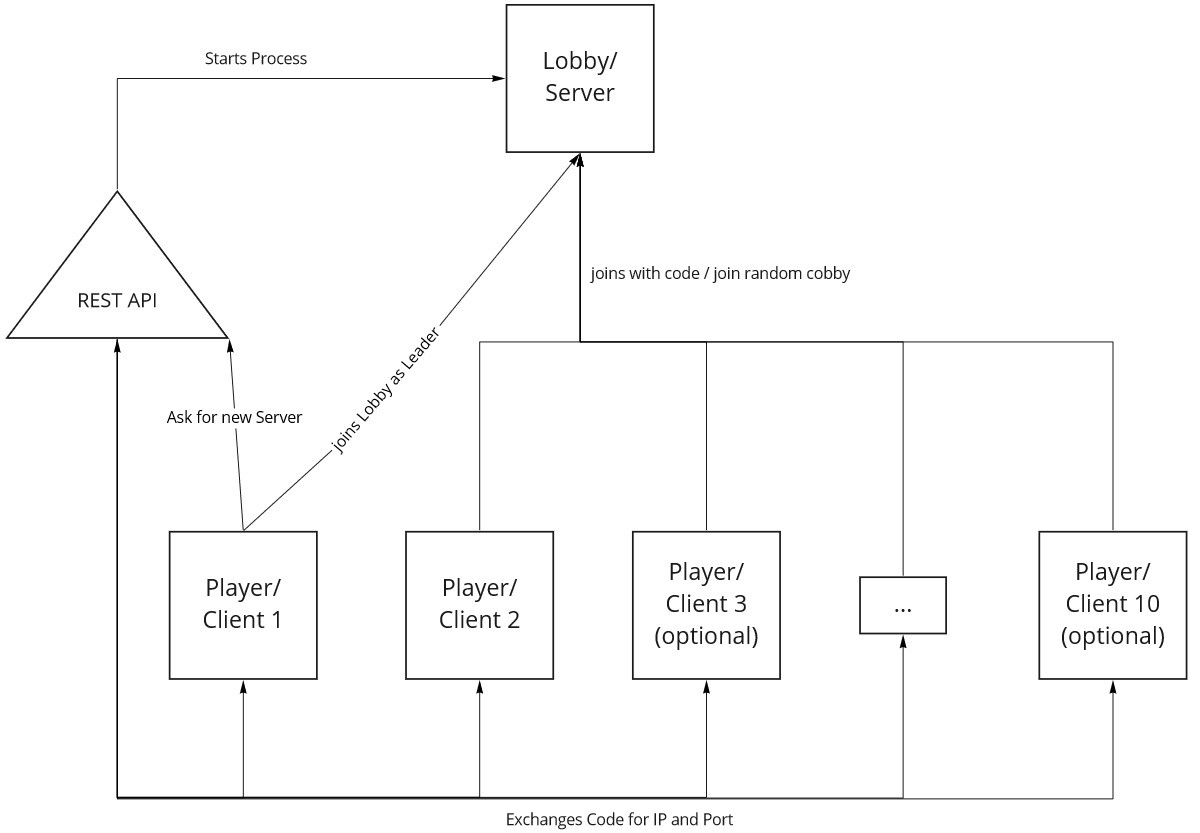
\includegraphics[width=100mm]{images/prototype_architecture_matchmaking.jpg}
	\caption[Architektur Matchmaking Diagramm]{Veranschaulichung der Architektur des Matchmakings im Prototyp}
	\label{pic:prototype_architecture_matchmaking}
\end{figure}

\textbf{Szenen:} \\
Im Prototyp gibt es lediglich 2 Szenen: Die Menü-Szene (Menu Scene) und die Spielszene (Game Scene).
Die Menu Scene gliedert sich in 2 verschiedene Sub-Menüs. Das 'Main Menu' wird zu Spielstart angezeigt und wenn ein Spieler die Verbindung zu einem Server abbricht oder verliert. Das 'Lobby Menu' wird angezeigt, sobald ein Spieler einer Lobby beigetreten ist. 

Die Game Scene wird geladen, sobald ein Spiel aus dem 'Lobby Menu' heraus gestartet wird. Das ist dann der Fall, wenn alle Mitglieder einer Lobby auf den Button 'Ready' gedrückt haben und der Leiter dieser Lobby auf den Button 'Start Game' gedrückt hat. 

\begin{figure}[H]
	\centering
	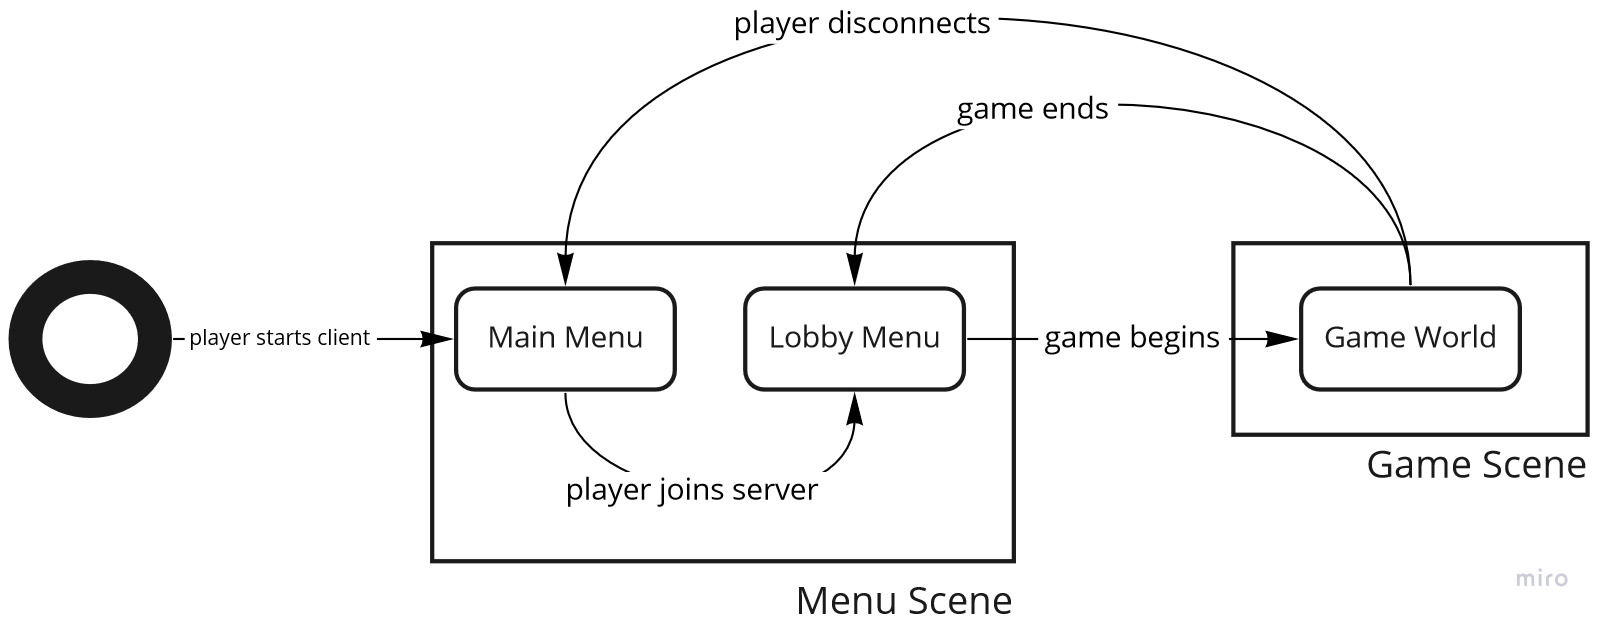
\includegraphics[width=90mm]{images/scene_architecture.jpg}
	\caption[Architektur Szenen Diagramm]{Veranschaulichung der Szenen-Architektur im Prototyp}
	\label{pic:scene_architecture}
\end{figure}

Auf die Implementierungen der einzelnen Konzepte wird in den kommenden Sektionen im Detail eingegangen. Die folgende Grafik zeigt die Relationen zwischen den implementierten Konzepten untereinander:

\begin{figure}[H]
	\centering
	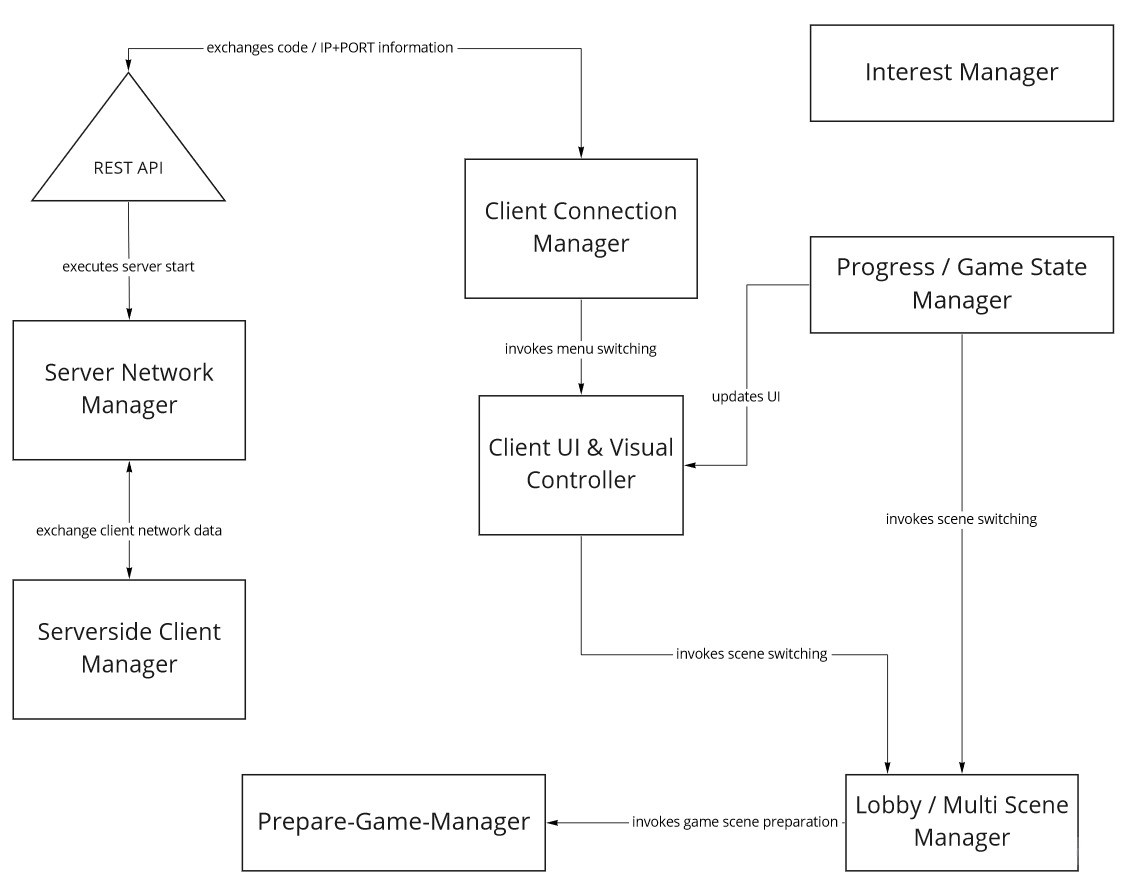
\includegraphics[width=90mm]{images/concept_relations.jpg}
	\caption[Architektur Konzept Relationen]{Veranschaulichung der Konzeptrelationen im Prototyp}
	\label{pic:concept_relations}
\end{figure}

\section{Implementierung: API für Matchmaking \& Server-Runner}

Für die Matchmaking- und Server-Runner API wurde auf eine externe Lösung zurückgegriffen, da eine eigene Entwicklung aus zeitlichen Gründen nicht möglich war. Genutzt wurde eine Lösung von Felix Brübach \cite{GitHub.20.02.2022}. Diese beinhaltet eine REST API, sowie eine Verwaltung von beliebig vielen Serverthreads. Diese werden repräsentiert durch eine Aneinanderreihung von einem Adjektiv und Tiernamen als 'Identifier'(ID). Dieser Identifier wird in dem Spielkonzept als 'Code' verwendet. Außerdem kann die REST API so konfiguiert werden, dass ein eigenes Datenmodell zusätzlich zu den IDs verwaltet wird. Die REST API erwartet ebenfalls eine Datei, welche sie zur Laufzeit als Server-Thread ausführen kann. Im Falle des Prototyps ist das eine Mirror Server-Instanz.

Die REST API akzeptiert die HTTP-Verben GET, POST, PUT und DELETE, mit denen server-relevante Daten abgefragt und Serverprozesse erzeugt, manipuliert, oder gelöscht werden können. Die Erzeugung der Serverprozesse erfolgt durch Ausführung der Mirror-Serverdatei mit Übergabe der folgenden 2 Programm-Argumente:

\begin{itemize}
	\item '--port': Die nächste freie Port-Nummer auf der Hardware, auf der auch die REST API läuft
	\item '--id': Die ID, welche die REST API für diesen Serverprozess erzeugt hat. Im Falle des Prototyps wird diese als 'Code' behandelt.
\end{itemize}

Der folgende Code (Vollständiger Code im Anhang) zeigt die Methode 'ServerStart', die innerhalb des Mirror-Serverprozesses aufgerufen wird, sobald die REST API den Prozess startet: 

\begin{lstlisting}[caption= OwnKcpTransport.cs ServerStart()]
public override void ServerStart()
{
	...
	int portIndex = Array.FindIndex(System.Environment.GetCommandLineArgs(), elem => elem == '--port') + 1;
	int codeIndex = Array.FindIndex(System.Environment.GetCommandLineArgs(), elem => elem == '--id') + 1;
	...
	port = Convert.ToUInt16(System.Environment.GetCommandLineArgs()[portIndex]);
	...
	lobbyCode = System.Environment.GetCommandLineArgs()[codeIndex];
	GameNetworkManager.singleton.curLobbyCode = lobbyCode;
	...
	base.server.Start(port);
}
\end{lstlisting}


\section{Implementierung: Client UI \& Visual Controller}
\label{implementierung:client_UI_Controller}

Der Client UI \& Visual Controller spielt im Prototyp eine wesentliche Rolle. Er kommt in der Game Scene als Singleton \cite{M.Gatrell.2009} zum Einsatz, wo er alle nötigen Methoden implementiert, um das lokale UI des Spielers manipulieren zu können. Hier sind nun 3 Beispiele aufgeführt:

Die folgende 'Update'-Methode ist eine von Unity bereitgestellte Schnittstelle. Der Rumpf der Update Methode ist nie vorgegeben und muss vom Entwickler selbst implementiert werden. Unity führt diese Methode jedes 'Frame' (Einzelbild \cite{Whaley.21.11.2018}) aus. Dies ermöglicht eine nahezu vollständige Echtzeitabfrage der Inputs (Tastatur / Maus / andere Eingangsgeräte) des Spielers. Es wird dauerhaft abgefragt, ob ein Spieler die Taste 'E' oder 'Q' auf seiner Tastatur drückt. Wenn er das tut und ebenfalls einige andere Randbedingungen erfüllt sind, wird ein 'Linksklick' auf den im UI des Spielers sichtbaren Button simuliert.

\begin{lstlisting}[caption= InGameUiControllerScript.cs Update Method]
private void Update()
{
	if (Input.GetKeyDown(KeyCode.E) && hotkeyImage != null && hotkeyImage.sprite == HOTKEY_KEYBOARD_E && interactButton.GetComponent<Button>().interactable )
	{
		interactButton.GetComponent<Button>().onClick.Invoke();
	}
	if (Input.GetKeyDown(KeyCode.Q) && lightButton.GetComponent<Button>().interactable)
	{
		lightButton.GetComponent<Button>().onClick.Invoke();
	}
}
\end{lstlisting}

\begin{figure}[H]
	\centering
	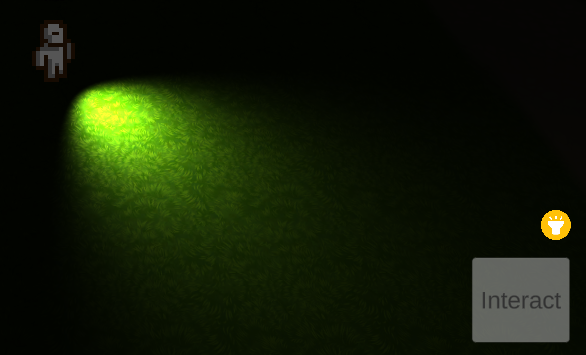
\includegraphics[width=120mm]{images/prototyp_interact_light_button.png}
	\caption[Interact and Light Button]{Der 'Interact' - und 'Light' Button im Client UI.}
	\label{pic:prototyp_interact_light_button}
\end{figure}

Doch was heißt das genau? Im folgenden Code wird ein Event definiert, welches durch andere Klassen 'abonniert' werden kann. Wird dann das Event durch '.Invoke()' ausgelöst, so werden alle Funktionen in externen Skripten ausgeführt, die dieses Event abonniert haben. Hier zunächst die Definition des Events im 'InGameUiControllerScript' und die Funktion 'clickInteractButton', die ausgeführt wird, wenn beispielsweise wie im obigen Code die Taste 'E' auf der Tastatur gedrückt wird.

\begin{lstlisting}[caption= InGameUiControllerScript.cs OnInteractButtonClick Event]
public event Action OnInteractButtonClick;	

public void clickInteractButton()
{
	OnInteractButtonClick?.Invoke();
}
\end{lstlisting}

Um den gesamten Aufrufstapel nachvollziehen zu können, folgt nun ein Beispiel aus einem anderen Script.
Die Klasse 'HiderScript.cs' abonniert in seiner Methode 'RpcEnableHideButton' das Event des InGameUiControllerScript Singletons 'OnInteractButtonClick' mit seiner eigenen Methode 'OnHiderHideButtonClick'. Die Methode 'RpcEnableHideButton' wird dann ausgeführt, wenn der Server einem Spieler mit der Rolle 'Hider' erlaubt, ein Versteck betreten zu dürfen.

\begin{lstlisting}[caption= HiderScript.cs Subscribe to InGameUiControllerScript Event]
[TargetRpc]
private void RpcEnableHideButton()
{
	InGameUiControllerScript.singleton.resetInteractButtonClickEvents();
	InGameUiControllerScript.singleton.OnInteractButtonClick += OnHiderHideButtonClick;
	InGameUiControllerScript.singleton.setInteractButtonEnabled(true);
	InGameUiControllerScript.singleton.setInteractButtonTextAndHotkeyImage('Hide');
}
\end{lstlisting}

\begin{figure}[H]
	\centering
	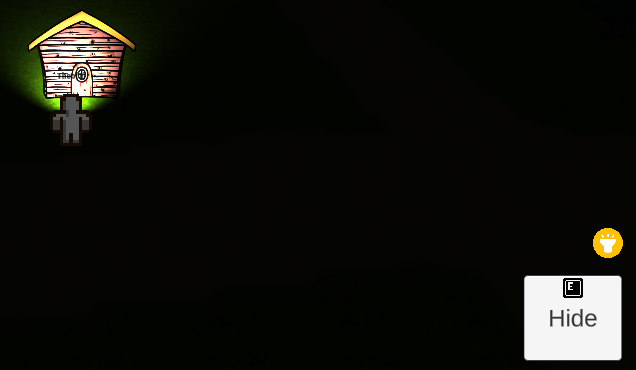
\includegraphics[width=120mm]{images/prototyp_hider_hide_button.png}
	\caption[Hider Hide Button]{Der 'Interact' Button nimmt die Funktion 'Hide' an.}
	\label{pic:prototyp_hider_hide_button}
\end{figure}

Sollte der Hider nun auf seinen 'Interact'-Button drücken, wird die folgende Methode 'OnHiderHideButtonClick' aufgerufen. Diese ruft eine weitere Methode 'CmdHideHider' auf, welche einen Mirror Remote Procedure Call\cite{.05.02.2022} zum Server darstellt.

\begin{lstlisting}[caption= HiderScript.csOnHiderHideButtonClick() Method]

[Client]
private void OnHiderHideButtonClick()
{
	if (enabled)
	{
		CmdHideHider();
	}
}

\end{lstlisting}

Der Server führt nun innerhalb des Methodenrumpfs von 'CmdHideHider' einige Überprüfungen durch, ändert Server-interne Variablen und sorgt somit dafür, dass alle Spieler darüber Bescheid wissen, dass sich der Spieler nun in einem Versteck befindet. (Vollständiger Code im Anhang)

\begin{lstlisting}[caption= HiderScript.cs Subscribe to InGameUiControllerScript Event]
	
[Command]
private void CmdHideHider()
{
	...
	RpcNotifyHideState(true, GameNetworkManager.singleton.getConfiguredPlayerSpeed());
	...
}	
\end{lstlisting}

Die nächste Beispielmethode implementiert die Logik, den Interact Button selbst aktiv und inaktiv zu setzen. Der Interact Button selbst verfügt ebenfalls über ein 'HotkeyImage', welches einem visuellen Indikator gleich kommt, der die aktuell zu drückende Taste auf der Tastatur darstellt. Dieser Indikator wird bei jedem Aufruf von 'setInteractButtonEnabled' ebenfalls an- oder ausgeschaltet.

\begin{lstlisting}[caption= InGameUiControllerScript.cs setInteractButtonEnabled]
public void setInteractButtonEnabled(bool enabled)
	{
		interactButton.GetComponent<Button>().interactable = enabled;
		if(hotkeyImage != null)
		hotkeyImage.gameObject.SetActive(enabled);
	}
\end{lstlisting}

Das letzte Beispiel ist eine Implementierung eines simplen 'Flip-Mechanismus' beim Betätigen des 'Light Buttons' (An- und ausschalten der Taschenlampe eines Spielers). Diese Logik tauscht lediglich das Bild (Sprite) aus, welches auf dem Button liegt.

\begin{lstlisting}[caption= InGameUiControllerScript.cs flipLightButtonImage]
public void flipLightButtonImage()
{
	if (!lightOn)
	{
		lightButton.GetComponent<Image>().sprite = lightOnSprite;
	}
	else
	{
		lightButton.GetComponent<Image>().sprite = lightOffSprite;
	}
	lightOn = !lightOn;
}
\end{lstlisting}


\section{Implementierung: Server Network Manager}

In der Implementierung des Prototyps ist der Server Network Manager ein Teil der 'GameNetworkManager' Klasse. Diese implementiert sowohl client- als auch serverseitige Netzwerkfunktionen. Die nicht vorhandene Separierung von Client- und Serverfunktionen ist dem Mirror Framework geschuldet. Die Klasse 'GameNetworkManager' ist ebenfalls ein Singleton und erbt von der Klasse 'NetworkManager', welche von Mirror bereitgestellt wird. Durch die Vererbung ist es möglich, virtuelle Methoden \cite{Billwagner.08.02.2022} der NetworkManager Klasse zu überschreiben, netzwerkseitige Events abzufangen und mit eigener Logik auf diese zu reagieren. 

Im folgenden Beispiel wird die virtuelle Methode 'OnServerConnect' überschrieben, um zu überprüfen, ob ein Spieler einer Spiel-Session beitreten darf. Sollte sich diese bereits in der Spiel-Szene befinden, wird eine neue Message erzeugt. Diese wird an den Client geschickt wird, der aktuell versucht, sich zu verbinden. Das struct 'Message' nutzt ein von Unity bereitgestelltes Interface 'NetworkMessage', welches eine leichtgewichtige Art und Weise der Netzwerk-Kommunikation ermöglicht. Das gleiche Schema wird im zweiten 'if' Block benutzt. Hier wird überprüft, ob die maximale Anzahl an Spielern innerhalb einer Lobby bereits erreicht ist. (Vollständiger Code im Anhang)

\begin{lstlisting}[caption= GameNetworkManager.cs OnServerConnect() und Message struct]

...	
public override void OnServerConnect(NetworkConnection conn)
{
	// If the game server is already in gameScene, forbid access to game
	if (singleton.getNetworkSceneName() == 'Assets/Scenes/GameScene.unity')
	{
		Message msg = new Message()
		{
			message = 'Game has already started',
			messageType = MessageType.gameAlreadyStartedError
		};
		conn.Send(msg);
		conn.Disconnect();
	}
	
	// Forbid access to a lobby, if the lobby is already at maxPlayers (configurable inside GameNetworkManager Component)
	if(lobbyPlayers.Count == maxPlayers)
	{
		Message msg = new Message()
		{
			message = 'Maximum Players reached for this lobby',
			messageType = MessageType.tooManyPlayersError
		};
		conn.Send(msg);
		conn.Disconnect();
	}
}
\end{lstlisting}

\begin{figure}[H]
	\centering
	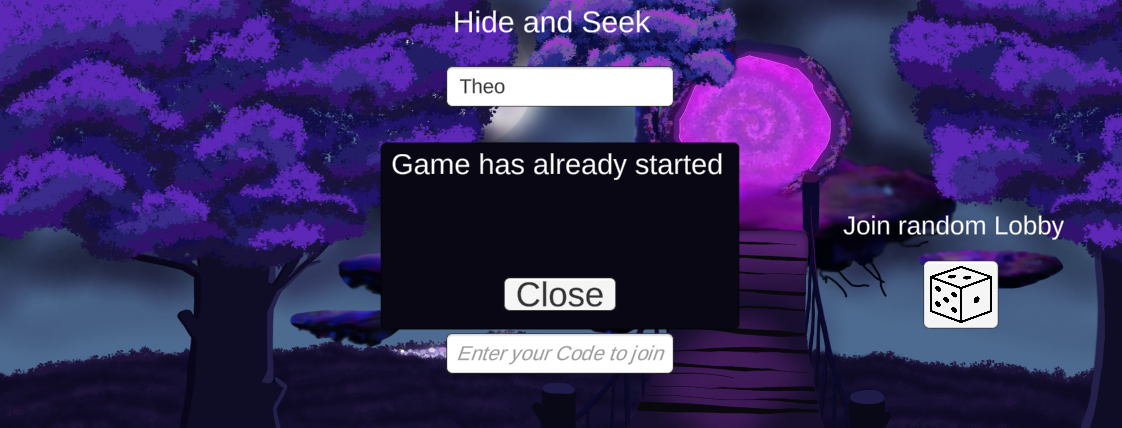
\includegraphics[width=120mm]{images/prototyp_game_has_already_started.png}
	\caption[Game has already started]{Ein Hinweis für einen Spieler, dass er dem Spiel nicht beitreten darf, da das Spiel bereits begonnen hat.}
	\label{pic:prototyp_game_has_already_started}
\end{figure}

Als Gegenstück zu 'OnServerConnect' gibt es ebenfalls die virtuelle Methode 'OnServerDisconnect', welche dann aufgerufen wird, wenn ein Spieler den Server gewollt oder ungewollt (bspw. durch Netzwerkabbruch) verlässt. Im Prototyp wurde diese Methode ebenfalls überschrieben und im GameNetworkManager selbst implementiert. 

Zunächst wird überprüft, ob die Anzahl aller Spieler, welche sich auf dem Server befinden, nach dem Beenden der aktuell abgefangenen und beendeten Client-Verbindung '0' beträgt. Falls ja, wird der Server-Prozess beendet. Sollten sich noch Spieler auf dem Server-Prozess befinden, werden je nach Spielszene verschiedene Szenarien durchlaufen. Wenn die Spielszene aktuell läuft, wird überprüft, ob die Anzahl an Spielern mit der Rolle 'Hider' oder 'Seeker' aktuell '0' beträgt. Falls einer der beiden Fälle zutrifft, wird das Spiel zugunsten des konkurrierenden Teams beendet. Wenn sich die Spiel-Session aktuell in der Menü-Szene befindet, werden Lobby-relevante Variablen aktualisiert und zunächst überprüft, ob der Spieler, welche gerade den Server verlassen hat, den Leader-Status hatte. Sollte dieser Fall zutreffen, wird der Leader-Status weiter gegeben. Zuletzt werden alle Spieler über den neuen Zustand der Lobby informiert. (Vollständiger Code im Anhang)

\begin{lstlisting}[caption= GameNetworkManager.cs OnServerDisconnect()]
public override void OnServerDisconnect(NetworkConnection conn)
{
	if ((NetworkServer.connections.Count == 0)
	{
		Debug.Log('Server shutdown because all Players left');
		Application.Quit();
	}
	...
	if(inGameProgressManager.getTotalSeekerCount() == 0)
	{
		inGameProgressManager.notifyHidersWinEvent();
	}

	if(inGameProgressManager.getTotalHidersCount() == 0)
	{
		inGameProgressManager.notifySeekerWinEvent();
	}
	...
}
\end{lstlisting}

Weitere virtuelle Methoden, welche der Prototyp implementiert hat, sind:

\begin{itemize}
	\item 'OnServerChangeScene' - diese Methode wird ausgeführt, sobald ein Szenenwechsel bevorsteht, aber noch nicht vollzogen ist.
	\item 'OnServerSceneChanged' - diese Methode wird ausgeführt, sobald ein Szenenwechsel vollständig vollzogen ist.
\end{itemize}

\section{Implementierung: Lobby / Multi Scene Manager}
\label{Lobby Manager Implementierung}

Das Spielkonzept beinhaltet, wie im Teil der \hyperref[Spielidee]{Spielidee} und \hyperref[Architektur]{Architektur} des Prototyps beschrieben, auch eine Lobbymechanik. Die Ideen aus dem Konzept des Lobby / Multi Scene Managers wurden aufgrund der geringen Anforderungen des Prototyps ebenfalls in der Klasse 'GameNetworkManager.cs' untergebracht. Dies hat den Vorteil, dass man die Lobby-spezifischen Variablen direkt mit den überschriebenen virtuellen Methoden der Mirror Klasse 'NetworkManager' kombinieren kann.

Im folgenden Beispiel werden die Server-internen Variablen aufgeführt, welche im Prototyp für die Szenen-übergreifende Lobby-Verwaltung verantwortlich sind:
    
\begin{enumerate}
	\item 'List<GameRule>' wird verwendet, um die für diesen Server-Prozess konfigurierten Spielregeln zu verwalten. Diese sind durch den Leader einer Lobby konfigurierbar. Beispiele für konfigurierbare Spielregeln sind:
	\begin{itemize}
		\item Total Game Time - nach wie vielen Sekunden wird das Spiel automatisch zu Gunsten der Spieler entschieden, welche zum Team 'Seeker' gehören.
		\item Player Base Speed - die Grundgeschwindigkeit der Spieler-Avatare.
		\item Daytime - eine Einstellung für den Wechsel zwischen Tag und Nacht.
	\end{itemize}
	\item 'LobbyPlayer leader' - beinhaltet das Spieler-Objekt, welches der Server als Leader einer Lobby ansieht.
	\item 'Dictionary<NetworkConnection, LobbyPlayer> lobbyPlayers' - in diesem Dictionary wird pro Spieler die dazugehörige 'NetworkConnection' Objekt und das 'LobbyPlayer' Spieler-Objekt verwaltet. 'NetworkConnection' ist eine Mirror-spezifische Klasse, welche alle Netzwerk-relevanten Informationen zu einem Spieler verwaltet (Bspw. die IP-Adresse oder eine für diesen Spieler einzigartige Verbindungs-ID).
	\item 'bool isLobbyReady' ist ein boolscher Wert, der nur dann den Wert 'true' annimmt, sobald alle Spieler durch das Drücken auf einen 'Ready'-Button signalisiert haben, dass sie bereit für den Wechsel in die Spiel-Szene sind.
	\item 'uint maxPlayers' ist ein Wert, der bestimmt, wieviele Spieler maximal einer Lobby beitreten dürfen.
	\item 'uint keepLobbyAliveTimeInSeconds' ist ein Wert, der festlegt, nach wie vielen Sekunden Inaktivität der Spieler ein Server-Prozess beendet wird.
\end{enumerate}

\newpage

\begin{lstlisting}[caption= GameNetworkManager.cs Lobby Variables]
	public List<GameRule> gameRules = new List<GameRule>();
	
	private LobbyPlayer leader = null;
	
	private Dictionary<NetworkConnection, LobbyPlayer> lobbyPlayers = 
	new Dictionary<NetworkConnection, LobbyPlayer>();
	
	private bool isLobbyReady = false;
	
	private uint maxPlayers = 10;
	private uint keepLobbyAliveTimeInSeconds = 600;
\end{lstlisting}

Die folgenden Methoden sorgen dafür, dass vor dem Übergang in die Spiel-Szene die nun nicht mehr benötigten Lobby-Spielerobjekte zerstört werden und im Anschluss der gewünschte Übergang in die Spiel-Szene erfolgt. Hierfür stellt Mirror die Methode 'ServerChangeScene' bereit, welche dafür sorgt, dass der Szenenwechsel sowohl beim Server, als auch bei allen verbundenen Clients vollzogen wird.

\begin{lstlisting}[caption= GameNetworkManager.cs StartGame]
public void StartGame()
{
	clearLobbyData();
	ServerChangeScene(gameScene);
}

private void clearLobbyData()
{
	foreach(LobbyPlayer lobbyPlayer in lobbyPlayers.Values)
	{
		NetworkServer.Destroy(lobbyPlayer.gameObject);
	}
}
\end{lstlisting}

Der Aufruf der Initialisierung des Szenenwechsels zurück in die Menü-Szene geschieht aus Komplexitätsgründen aus dem InGameProgressManager heraus. Die nähere Erläuterung folgt in der Sektion \hyperref[Progress Manager]{'Implementierung: Progress / Game-State Manager'}.

\section{Implementierung: Client Connection Manager}

Die Prinzipien des Client Connection Manager Konzepts wurden im Prototyp innerhalb der Klasse 'ConnectionScript.cs' realisiert. Die Hauptaufgabe ist der Kommunikationsaustausch mit der Matchmaking API sowie der Verbingdungsaufbau zu einer Mirror-Serverinstanz. Für diesen Kommunikationsaustausch wurde das Open Source Package 'Rest Client' von Juan Nicholls (proyecto26) benutzt \cite{GitHub.10.02.2022}.

Im folgenden Code Beispiel wird zunächst das Datenmodell einer Lobby aus der Sicht der Matchmaking API und dem 'ConnectionScript' aufgezeigt. Eine kurze Erläuterung der einzelnen Felder:

\begin{itemize}
	\item 'bool isPublic' sagt aus, ob eine Lobby öffentlich bereitgestellt wurde. Falls ja, können andere Spieler auch ohne Zugangscode über die 'Join Random Lobby' Funktion des Prototyps dieser Lobby beitreten.
	\item 'string address' gibt die IP-Adresse des Servers an, auf dem die der Mirror-Serverprozess zu dieser Lobby gestartet wurde.
	\item 'int port' gibt den Port des Mirror-Serverprozesses an, den der Server für diesen Prozess reserviert hat.
	\item 'string code' enthält einen Zugangsschlüssel, den Clients nutzen können, um im Austausch mit der Matchmaking API das passende Lobbyobjekt zu erhalten, mit dem sie sich dann (mithilfe des address + port Felds) ebenfalls auf den gleichen Mirror-Serverprozess verbinden können.
\end{itemize}

\begin{lstlisting}[caption= ConnectionScript.cs Matchmaking Data]
// The Data which is necessary for describing a lobby. This Information is synchronized between the REST API and the Mirror Server & Client
private class Lobby
{
	public bool isPublic;
	public string address;
	public int port;
	public string code;
}

private class PublicLobbys
{
	public Lobby[] lobbys;
}
\end{lstlisting}

\begin{figure}[H]
	\centering
	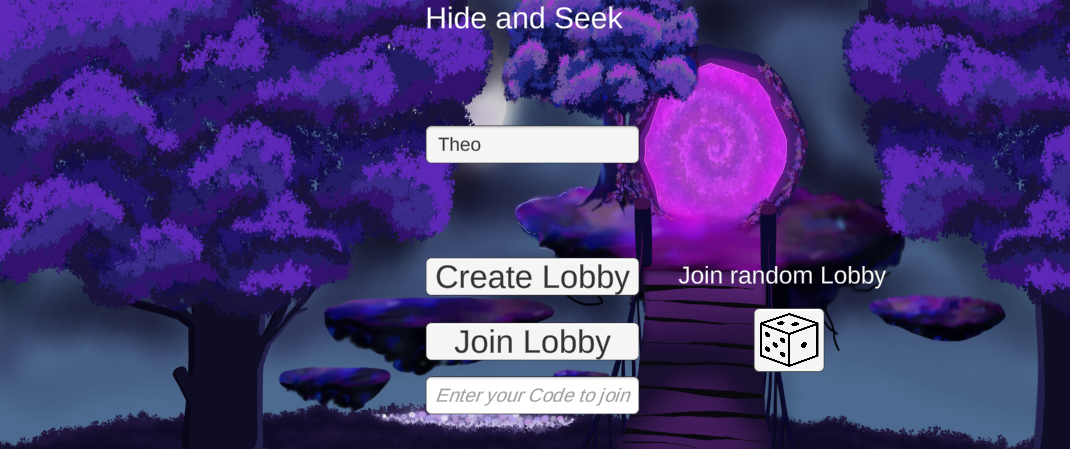
\includegraphics[width=120mm]{images/prototyp_main_menu.png}
	\caption[Prototyp Main Menu]{Das Main Menu dient hauptsächlich zur Verbindungsherstellung zu einem Server}
	\label{pic:prototyp_main_menu}
\end{figure}

Sollte ein Spieler im Hauptmenü auf den Button 'Create Lobby' drücken, so wird eine POST Anfrage an die Matchmaking API geschickt. Diese liefert ein neu erzeugtes Lobbyobjekt zurück, mit dem sich der Spieler auf den neu erzeugten Mirror-Serverprozess verbindet. Folgender Code zeigt die Implementierung:

\newpage

\begin{lstlisting}[caption= ConnectionScript.cs createLobby()]
private void createLobby()
{
	RestClient.Post<Lobby>(apiBaseUrl + '/v0/lobbies', '{\'isPublic\': true}').Then(lobby =>
	{
		string[] splitAddress = lobby.address.Split(new string[] { '://' }, StringSplitOptions.None);
		
		GameNetworkManager.singleton.StartClient(new UriBuilder(splitAddress[0], splitAddress[1], lobby.port).Uri);
	}).Catch(error =>
	{
		onFailure();
		Debug.LogError('Error when creating lobby: ' + error);
	});
}	
\end{lstlisting}

Im Fall, dass ein Spieler auf den Button 'Join Lobby' drückt, wird die Zeichenkette, die der Nutzer in das entsprechende 'Code-Input-Feld' eingegeben hat, der Methode 'joinWithCode' übergeben. Diese überprüft zunächst, ob der Spieler keinen Code eingegeben hat. Falls die übergebene Zeichenkette nicht leer ist, führt das 'ConnectionScript' eine GET Anfrage an die Matchmaking API aus, die intern überprüft, ob eine Lobby mit diesem Zugangsschlüssel existiert. Falls dies der Fall ist, verbindet sich der Spieler automatisch mit der entsprechenden Lobby. (Vollständiger Code im Anhang)

\begin{lstlisting}[caption= ConnectionScript.cs joinWithCode()]
private void joinWithCode(string code)
{
	...		
	RestClient.Get<Lobby>(GameNetworkManager.singleton.frapiBaseUrl + '/v0/lobbies/' + code).Then(lobby =>
	{
		string[] splitAddress = lobby.address.Split(new string[] { '://' }, StringSplitOptions.None);
		GameNetworkManager.singleton.StartClient(new UriBuilder(splitAddress[0], splitAddress[1], lobby.port).Uri);
	}).Catch(error =>
	{
		Debug.LogError('Error when joining lobby: ' + error);
		onFailure();
	}
}
\end{lstlisting}

Sollte sich ein Spieler über 'Create Lobby' oder 'Join Lobby' erfolgreich zu einer (neuen) Serverinstanz verbunden haben, findet sich dieser Spieler im 'Lobby Menu' wieder:

\begin{figure}[H]
	\centering
	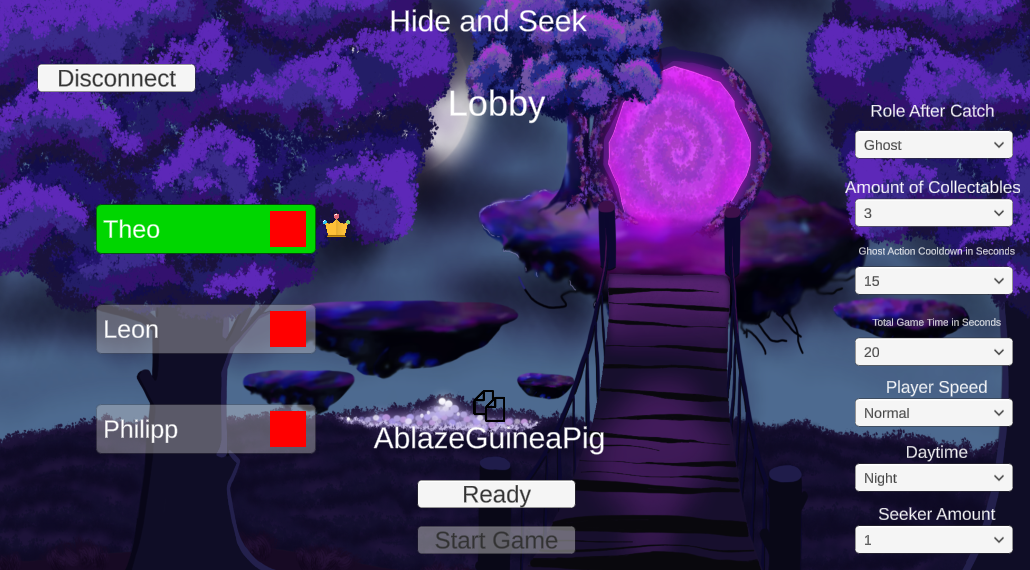
\includegraphics[width=120mm]{images/prototyp_lobby_menu.png}
	\caption[Prototyp Lobby Menu]{Eine offene Lobby mit 3 Spielern}
	\label{pic:prototyp_lobby_menu}
\end{figure}

In den beiden obigen Beispielen wird beim Auslösen des Catch-Falls die Methode 'onFailure' aufgerufen. Dieser Fall tritt bei verschiedenen Szenarien ein. Beispielsweise, wenn die Kommunikation mit der REST API nicht möglich ist, oder diese einen 4XX oder 5XX HTTP-Status-Code liefert. Die Methode sorgt dafür, dass der Nutzer zurück ins Main-Menü geschickt wird und ihm eine Nachricht angezeigt wird, dass der Verbindungsversuch gescheitert ist.

\begin{lstlisting}[caption= ConnectionScript.cs onFailure()]
private void onFailure()
{
	unregisterCallbacks();
	GameNetworkManager.singleton.curNetworkMessage.message = 'Network Error: Could not Connect to Server';
	changeToMainMenu(true);
}

\end{lstlisting}

Die Implementierung einer 'onSuccess' Funktion (das Gegenstück zu 'onFailure') innerhalb des Connection-Managers ist nicht nötig, da bei erfolgreicher Verbindungsherstellung Mirror-spezifische Events und Handler-Funktionen für die weitere Logik sorgen. Diese sind nicht mehr Teil des 'ConnectionScript'.

\section{Implementierung: Serverside Client Manager}

Das Konzept des Serverside Client Managers wird nahezu vollständig durch mirrorinterne Prozesse gelöst. Die Verwaltung aller Clients geschieht durch die 'GameNetworkManager' Klasse, welche von der Mirror Klasse 'NetworkManager' erbt. Die Superklasse 'NetworkManager' wiederum nutzt eine andere Mirror-Klasse 'NetworkServer', diese beinhaltet ein Dictionary, das die Verbindungen zu allen Clients verwaltet. Im folgenden Code ist das Dictionary und die dazu gehörenden Methoden 'AddConnection' und 'RemoveConnection' zu sehen. (Vollständiger Code im Anhang)

\begin{lstlisting}[caption= Mirror Class NetworkServer.cs Connection Handling]
...
public static Dictionary<int, NetworkConnectionToClient> connections = new Dictionary<int, NetworkConnectionToClient>();
...
public static bool AddConnection(NetworkConnectionToClient conn)
{
	...
	connections[conn.connectionId] = conn;
	...
}
...
public static bool RemoveConnection(int connectionId)
{
	return connections.Remove(connectionId);
}
\end{lstlisting}

In der aktuellen Version des Prototyps werden spielerbezogene 'Sonderinformationen', wie Spielername und Rolle, im 'GameNetworkManager' mitverwaltet. Die Aufgabe des Serverside Client Managers wird in der Komponente, die in der Sektion \hyperref[Lobby Manager Implementierung]{'Implementierung: Lobby / Multi Scene Manager'} beschrieben wird, mitverwaltet. 

Diese Tatsache ist allerdings an die Randbedingung geknüpft, dass für den Prototypen das Mirror Framework genutzt wurde, welches viele Funktionen auf die überschriebene 'NetworkManager' Klasse abwälzt. Außerdem speichert der Prototyp keine große Anzahl an 'Sonderinformationen' (wie Charakterindividualisierung, Account-Informationen / In-Game-Shop Daten etc.). Da der Komplexitätsaufwand für eine gesonderte Handhabung dieser Informationen bei steigenden Anforderungen enorm zunimmt, ist es ratsam, die Komponente 'Serverside Client Manager' gesondert zu implementieren.

\section{Implementierung: Prepare-Game-Manager}
\label{Implementierung:prepare_game_manager}

Die Klasse 'PrepareGameManager' sorgt innerhalb des Prototypen dafür, dass anhand der vom Lobbyleiter konfigurierten Anzahl an Objekten eine entsprechende Menge an zufällig ausgewählten 'Collectable'-Objekten im Spielfeld platziert werden. Anschließend wählt der 'PrepareGameManager' zufällig eines von drei, für dieses spezifische 'Collectable'-Objekt möglichen 'Destination'-Objekten aus, welches als Zielpunkt dient. Die folgende Methode 'spawnObjects' führt diese Logik aus. (Vollständiger Code im Anhang)

\begin{lstlisting}[caption= PrepareGameManager.cs Variablen und spawnObjects()]
...
private void spawnObjects()
{	
	...	
	GameObject curCollectableGameObject = popCollectableObjectAt(randomIndex);
	GameObject collectInstance = Instantiate(curCollectableGameObject, curCollectableSpawnPoint.position, curCollectableSpawnPoint.rotation);
	NetworkServer.Spawn(collectInstance);
	...
	GameObject curDestinationObject = relatedDestinationObjects[randomRelatedDestinationObjectPickIndex];
	GameObject destinationInstance = Instantiate(curDestinationObject, curDestinationSpawnpoint.position, curDestinationSpawnpoint.rotation);
	NetworkServer.Spawn(destinationInstance);
	...
}
\end{lstlisting}

\begin{figure}[H]
	\centering
	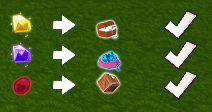
\includegraphics[width=60mm]{images/prototyp_task_list.png}
	\caption[Initial Task List]{Gespawnte 'Collectable' und 'Destination' Objekte werden den Spielern innerhalb einer Liste angezeigt.}
	\label{pic:prototyp_task_list}
\end{figure}

Der 'PrepareGameManager' sorgt außerdem für die Verwaltung der Spawn-Punkte aller Spieler. Innerhalb der Variable 'possiblePlayerSpawnPoints' werden diese gespeichert. Die Methode 'fillPossiblePlayerSpawnPoints' sorgt dafür, dass die Variable mit Werten gefüllt wird.

\begin{lstlisting}[caption= PrepareGameManager.cs fillPossiblePlayerSpawnPoints()]
private List<Transform> possiblePlayerSpawnPoints;

public void fillPossiblePlayerSpawnPoints()
{
	possiblePlayerSpawnPoints = new List<Transform>();
	GameObject[] portals = GameObject.FindGameObjectsWithTag('Portal');
	foreach (GameObject portal in portals)
	{
		possiblePlayerSpawnPoints.Add(portal.transform);
	}
}
\end{lstlisting}

Die Methode 'popRandomPlayerSpawnPoint' gibt einen zufälligen Spieler-Spawnpunkt zurück und entfernt ihn von der Liste der noch möglichen Spieler-Spawnpunkte.

\begin{lstlisting}[caption= PrepareGameManager.cs popRandomPlayerSpawnPoint()]
public Transform popRandomPlayerSpawnPoint()
{
	int randomIndex = new Random().Next(possiblePlayerSpawnPoints.Count);
	Transform result = possiblePlayerSpawnPoints[randomIndex];
	possiblePlayerSpawnPoints.Remove(possiblePlayerSpawnPoints[randomIndex]);
	return result;
}
\end{lstlisting}

Aufgerufen wird die Methode 'popRandomPlayerSpawnPoint' innerhalb der \hyperref[Lobby Manager Implementierung]{Lobby Manager Implementierung} in der Methode 'replaceLobbyPlayersWithGamePlayers'. In dieser Methode werden alle Lobby-Spielerobjekte mit InGame-Spielerobjekten (Charakteren) ersetzt. Unter anderem wird in diesem Ersetzungsprozess der neue, zufällige Spawn-Punkt benötigt, der 'popRandomPlayerSpawnPoint' liefert. (Vollständiger Code im Anhang)

\begin{lstlisting}[caption= GameNetworkManager.cs replaceLobbyPlayersWithGamePlayers()]
private void replaceLobbyPlayersWithGamePlayers()
{
		...
		Transform spawnPoint = prepareGameManager.popRandomPlayerSpawnPoint();
		Vector3 spawnPosition = new Vector3(spawnPoint.position.x, 0.88f, spawnPoint.position.z);
		GameObject gamePlayerInstance = Instantiate(gamePlayerPrefab, spawnPosition, spawnPoint.rotation);
		...
}
\end{lstlisting}


\section{Implementierung: Progress / Game-State Manager}
\label{Progress Manager}

Das Konzept des Progress / Game State Managers wurde innerhalb des Prototyps als Klasse 'InGameProgressManager' realisiert. Dieser verwaltet einen globalen Timer (Stoppuhr), der beim Erreichen des Wertes '0' das Spiel automatisch für die Gruppe der Spieler mit der Rolle 'Seeker' beendet.

Der folgende Code zeigt, wie der globale Timer gestartet wird. Die Methode 'startGameTimer' wird serverseitig ausgeführt, sobald ein Szenenwechsel in die Spiel-Szene erfolgt. Außerdem wird beim Starten des Timers eine Netzwerk-Nachricht initialisiert, die bei jedem 'Tick' des Timers an alle Clients gesendet wird. Diese Nachricht enthält die Information, wie viele Sekunden noch übrig sind. Ein 'Tick' entspricht dem Ablauf einer Sekunde. (Vollständiger Code im Anhang)

\begin{lstlisting}[caption= InGameProgressManager.cs global Game Time Handling]
...
public void startGameTimer(uint totalGameTime)
{
	...
	gameTimer = new Timer(1f, totalGameTime, handleTick);
	TimersManager.SetTimer(this, gameTimer);
	...
}

private void handleTick()
{
	...
	countDownGameTime();
	...
}

private void countDownGameTime()
{
	curGameTimeLeftMsg.message = 'Game Time Left: ' + Math.Round(gameTimer.RemainingTime());
	
	// Notify each client about the server sided game time left
	foreach (var conn in NetworkServer.connections)
	{
		conn.Value.Send(curGameTimeLeftMsg);
	}
}
\end{lstlisting}

\begin{figure}[H]
	\centering
	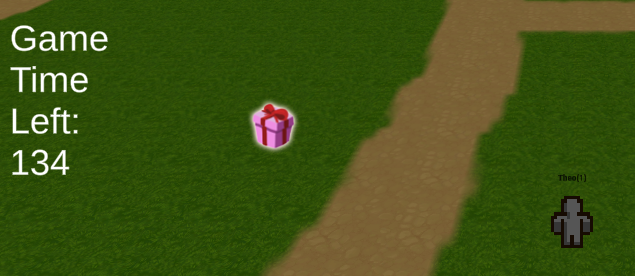
\includegraphics[width=60mm]{images/prototyp_game_timer.png}
	\caption[Time Left Counter]{Den Spielern wird der Timer im UI angezeigt.}
	\label{pic:prototyp_game_timer}
\end{figure}

Darüber hinaus speichert der 'InGameProgressManager' die Information, wie viele 'Collectable' Objekte die Spielergruppe mit der Rolle 'Hider' bereits zu ihrem Ziel gebracht haben. Erreicht die Variable 'totalDeliveredItems' den Wert, den der Lobbyleiter innerhalb der Lobby Szene konfiguriert hat, hat die Spielergruppe mit der Rolle 'Hider' die Spielrunde gewonnen.

\begin{lstlisting}[caption= InGameProgressManager.cs Item Devlivery Handling]
private ushort totalDeliveredItems = 0;

public void incrementTotalDeliveredItems()
{
	totalDeliveredItems++;
	if(totalDeliveredItems >= (GameNetworkManager.singleton.getConfiguredCollectableItemsSetting()))
	{
		notifyHidersWinEvent();
	}
}	
\end{lstlisting}

\begin{figure}[H]
	\centering
	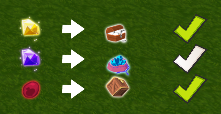
\includegraphics[width=60mm]{images/prototyp_task_list_progress.png}
	\caption[Updated Task List]{Sobald ein Item abgegeben wurde, wird der Haken in der entsprechenden Zeile in der Task-Liste grün.}
	\label{pic:prototyp_task_list_progress}
\end{figure}

Ist das Spiel für eine Partei gewonnen, gibt der 'InGameProgressManager' die Information an alle Clients per Netzwerk-Nachricht weiter und leitet die serverseitigen Konsequenzen ein. Der folgende Code zeigt den Code eines Sieges für die Spielergruppe 'Hider': 

Der Aufruf von 'StartCoroutine(endGameCoroutine())' ermöglicht innerhalb der 'IEnumerator endGameCoroutine' Funktion ein aktives Warten beim Ausführen von 'yield return new WaitForSeconds(2f);'. Die Übergabe des Parameters '2f' sorgt für eine Wartezeit von exakt 2 Sekunden. Der Grund für das aktive Warten ist die clientseitige Verarbeitung der Netzwerk-Nachricht, die in der Funktion 'notifyHidersWinEvent' geschickt wird. Alle Clients bekommen einen visuellen Indikator im User-Interface angezeigt, der die Information beinhaltet, welche Spielergruppe die aktuelle Runde gewonnen hat. Ohne das aktive Warten auf dem Server würden alle Spieler unmittelbar nach Spielende sofort in die Menü-Szene zurückgeworfen werden.

\begin{lstlisting}[caption= InGameProgressManager.cs Win Event]
	
public void notifyHidersWinEvent()
{
	winMsg = new Message()
	{
		message = 'Hiders won the Game',
		messageType = MessageType.hidersWinNotification
	};
		
	foreach (var conn in NetworkServer.connections)
	{
		conn.Value.Send(winMsg);
	}	
	StartCoroutine(endGameCoroutine());
}

IEnumerator endGameCoroutine()
{
	resetInGameProgressManager();
	gameTimer.SetPaused(true);
	disablePlayerMovementGlobal();
	
	yield return new WaitForSeconds(2f);
	GameNetworkManager.singleton.ServerChangeScene(GameNetworkManager.singleton.offlineScene);
}

\end{lstlisting}

\begin{figure}[H]
	\centering
	
\includegraphics[width=80mm]{images/prototyp_hiders_won.png}
	\caption[Hiders won the game]{Visueller Indikator, um allen Spielern zu zeigen, dass das Team 'Hider' gewonnen hat.}
	\label{pic:prototyp_hiders_won}
\end{figure}

\section{Nicht implementierte Konzepte}
\textbf{Runtime Spawn Manager:}

Das Spielkonzept hat nicht vorausgesetzt, dass nach Initialisierung der Spiel-Szene weitere Objekte gespawnt werden müssen. Jegliche Objekte, die für eine Spiel-Session benötigt werden, spawnt der \hyperref[Implementierung:prepare_game_manager]{'Prepare-Game-Manager'} bereits zum Szenenwechsel zwischen Menü-Szene und Spiel-Szene. Aus diesem Grund wurde für den Prototypen auf den Runtime Spawn Manager verzichtet.

\textbf{Interest Manager:}

Mirror bietet eine Reihe an Komponenten an, die eine eigene Implementierung eines Interest Managers überflüssig machen. Für den Prototypen wurde die Komponente 'Team Interest Management' benutzt \cite{.17.02.2022b}. Diese sorgt dafür, dass (Spieler)-Objekte nur für die Mitglieder einer Gruppe sichtbar sind. Im Falle des Prototyps sollen Spieler mit der Rolle 'Ghost' lediglich für Spieler mit der Rolle 'Hider' und 'Ghost' sichtbar sein. Spieler mit der Rolle 'Seeker' sollen Spieler mit der Rolle 'Ghost' nicht sehen können.

Sollte ein Spielkonzept jedoch Voraussetzungen besitzen, die über die Möglichkeiten der vordefinierten Interest Manager Komponenten von Mirror hinausgehen, so bietet Mirror ebenfalls die Möglichkeit, eigene Interest Manager Implementierungen zu erstellen, indem Mirror eine abstrakte Klasse 'InterestManagement' bereitstellt. Falls eine eigene Interest Manager Klasse von dieser erbt, kann sie die Methoden 'OnCheckObserver' und 'OnRebuildObservers' überschreiben\cite{.17.02.2022c}. 

\begin{itemize}
	\item 'OnCheckObserver' wird aufgerufen, wenn ein neuer Spieler spawnt. Gibt 'true' zurück, wenn ein (Spieler)-Objekt von dem neu gespawnten Spieler gesehen werden kann.
	\item 'OnRebuildObservers' wird innerhalb einer Update-Methode (diese wurde bereits in der Sektion \hyperref[implementierung:client_UI_Controller]{'Implementierung: Client UI \& Visual Controller'} erklärt) aufgerufen. Diese sorgt dafür, dass die Sichtbarkeit aller gespawnten Objekte neu berechnet wird.
\end{itemize}